\documentclass[convert={density=5000,size=1080x800,outext=.png}]{standalone}

\usepackage{tikz}
\usepackage{xcolor}

\usetikzlibrary{matrix}

\begin{document}
\pagecolor[RGB]{255,255,254}
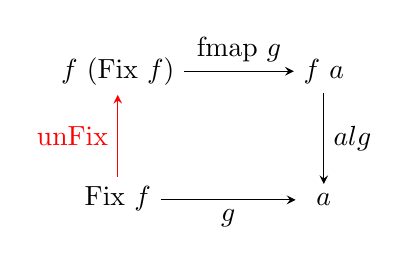
\begin{tikzpicture}
\matrix (m) [matrix of math nodes,row sep=3em,column sep=4em,minimum width=2em]
{
   f\ (\mbox{Fix}\ f) & f\ a \\
   \mbox{Fix}\ f & a \\
};
\path[-stealth]
  (m-1-1) edge node [above] {$\mbox{fmap}\ g$} (m-1-2)
  (m-2-1) edge [red] node [left] {$\mbox{unFix}$} (m-1-1) 
  (m-2-1.east|-m-2-2) edge node [below] {$g$} (m-2-2)
  (m-1-2) edge node [right] {$alg$} (m-2-2);
\end{tikzpicture}
\end{document}
